\section{Evaluation}
\FloatBarrier%

\subsection{Regularisation}
Since regularisation is very important to prevent overfitting, the common
methods of regularisation are tested first to obtain a good baseline value for the
rest of the experiments. These methods are:
\begin{itemize}
  \item Dropout, with values taken from the set
    $\left\{0.0, 0.1, 0.2, 0.3, 0.4, 0.5\right\}$.
  \item Weight decay, with values taken from the set
    \[\left\{0.0, \num{1e-5}, \num{1e-4}, \num{1e-3}, \num{1e-2},
    \num{1e-1}\right\}.\]
\end{itemize}
Further details on these methods are given in \cref{sec:method}.

\subsubsection{Dropout}
\Cref{fig:dropout_plots} shows the training loss over time, as well as the
resulting precision-recall curve on the training set. Other than the training
loss being higher with higher dropout values (which is to be expected), there
does not seem to be any difference in performance. This lack of effect is
also shown in \cref{fig:dropout_dists}. If anything, no dropout appears to have
the best performance by a slight margin, although none of the distributions are
different in a statistically significant way. The full data, with the mean and
standard deviation of the F1 score and the area under the curve, are given in
\cref{tbl:dropout}.

\begin{figure}[htbp]
  \centering
  \begin{subfigure}[t]{0.49\textwidth}
    \centering
    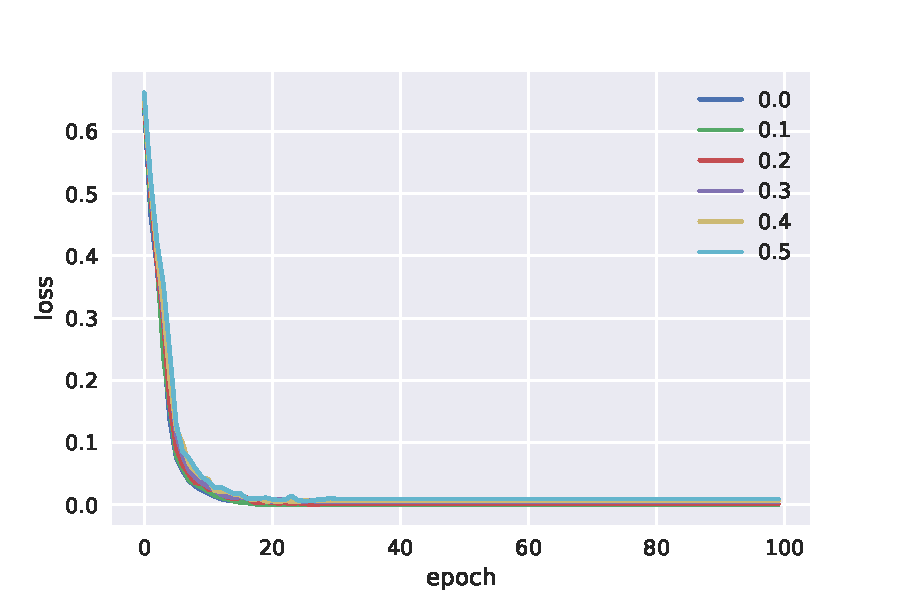
\includegraphics[width=\textwidth]{./figures/results/dropout/losses.pdf}
    \caption{The average loss at each epoch.\\}%
    \label{fig:dropout_loss}
  \end{subfigure}
  \begin{subfigure}[t]{0.49\textwidth}
    \centering
    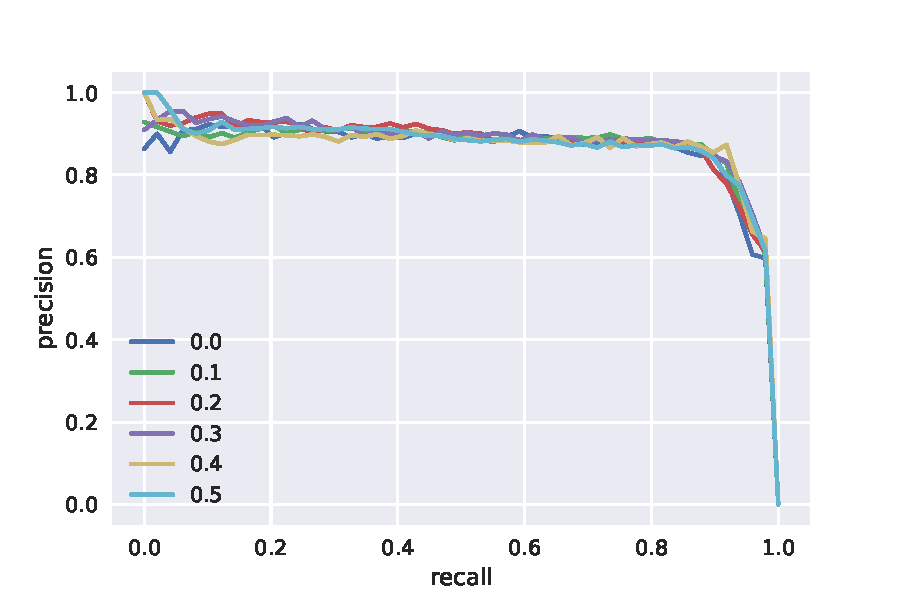
\includegraphics[width=\textwidth]{./figures/results/dropout/pr.pdf}
    \caption{The average precision-recall curves at various dropout values.}%
    \label{fig:dropout_pr}
  \end{subfigure}
  \caption{The loss over time (\subref{fig:dropout_loss}) and the
    precision-recall curve (\subref{fig:dropout_pr}). In both cases, the values are
    averaged over 10 trials.}%
    \label{fig:dropout_plots}
\end{figure}

\begin{figure}[htbp]
  \centering
  \begin{subfigure}[t]{0.49\textwidth}
    \centering
    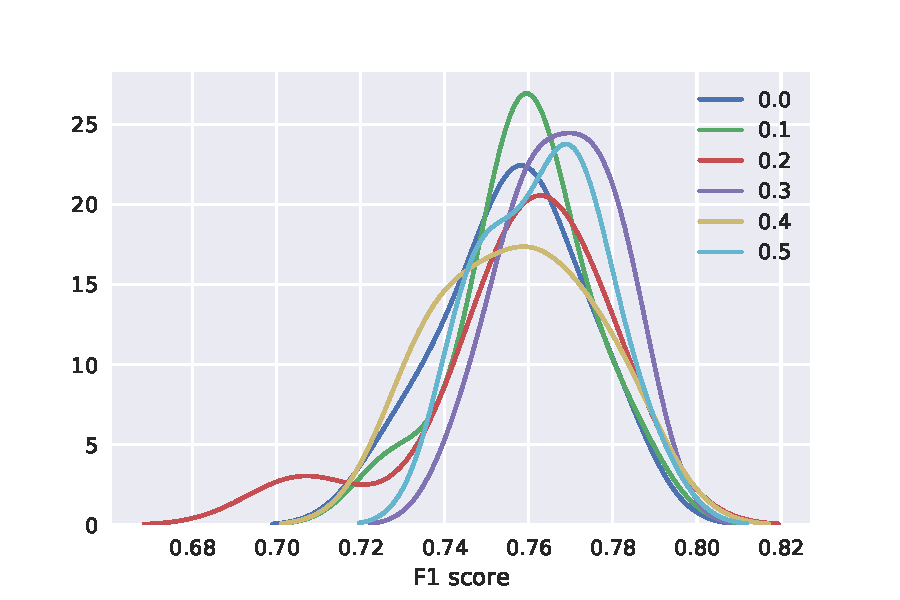
\includegraphics[width=\textwidth]{./figures/results/dropout/kde_f1.pdf}
    \caption{Kernel density estimation}%
    \label{fig:dropout_kde}
  \end{subfigure}
  \begin{subfigure}[t]{0.49\textwidth}
    \centering
    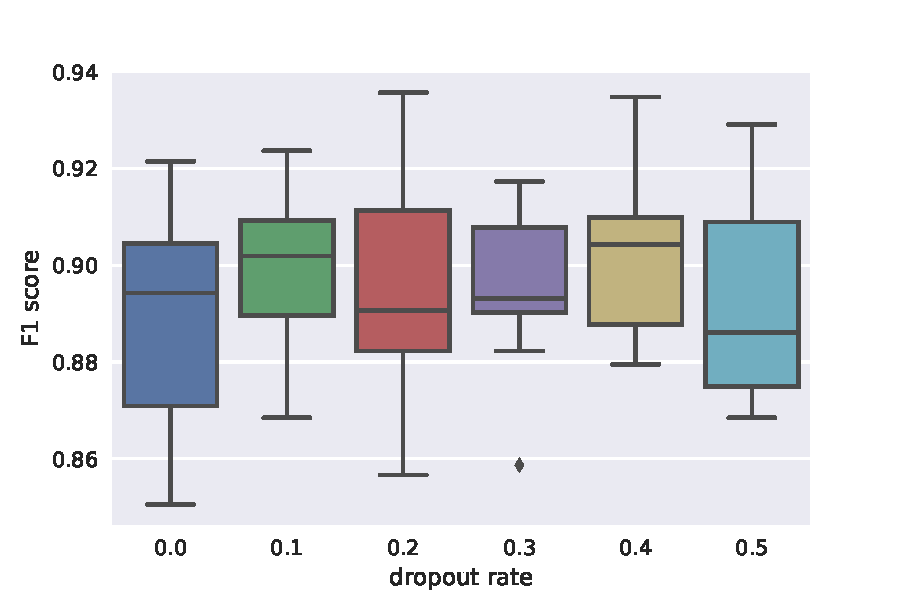
\includegraphics[width=\textwidth]{./figures/results/dropout/boxplot_f1.pdf}
    \caption{Boxplot}%
    \label{fig:dropout_box}
  \end{subfigure}
  \caption{A kernel density estimation and boxplot, based on the F1 score values
  over 10 repeated trials.}%
  \label{fig:dropout_dists}
\end{figure}

\begin{table}[htb]
  \centering
  \import{./figures/results/dropout/}{scores.tex}
  \caption{The F1 and AoC scores at various dropout values.}%
  \label{tbl:dropout}
\end{table}

\FloatBarrier%
\subsubsection{Weight decay}
Similarly to the dropout plots, \cref{fig:decay_plots} shows the training loss
over time and the precision-recall curve at various weight decay values. It is
immediately obvious that with a (frankly absurdly high) value of \num{1e-1}, the
model has trouble converging to a minimum. This effect is present but less
pronounced with the value of \num{1e-2}. In spite of this, the precision-recall
curve shows the model with a decay of \num{1e-2} clearly rising above the rest.
The distribution of the F1 scores in \cref{fig:decay_dists} tells a similar
story, with the \num{1e-2} model's distribution barely even overlapping with the
others. \Cref{tbl:decay_p} gives the \emph{p}-values for the probability of each
distribution being the same (i.e.\ the chance of the null hypothesis that two
sets of results are generated from the same underlying distribution being true).
Looking at this in combination with \cref{fig:decay_kde} and taking the standard
practice of rejecting the null hypothesis when $p < 0.05$, any value for the
decay parameter equal to or greater than \num{1e-3} performs better than no
decay in a statistically significant manner. In addition, a value of \num{1e-2}
clearly outperforms the other values with incredible certainty. The raw numbers
are shown in \cref{tbl:decay}.

\begin{figure}[htbp]
  \centering
  \begin{subfigure}[t]{0.49\textwidth}
    \centering
    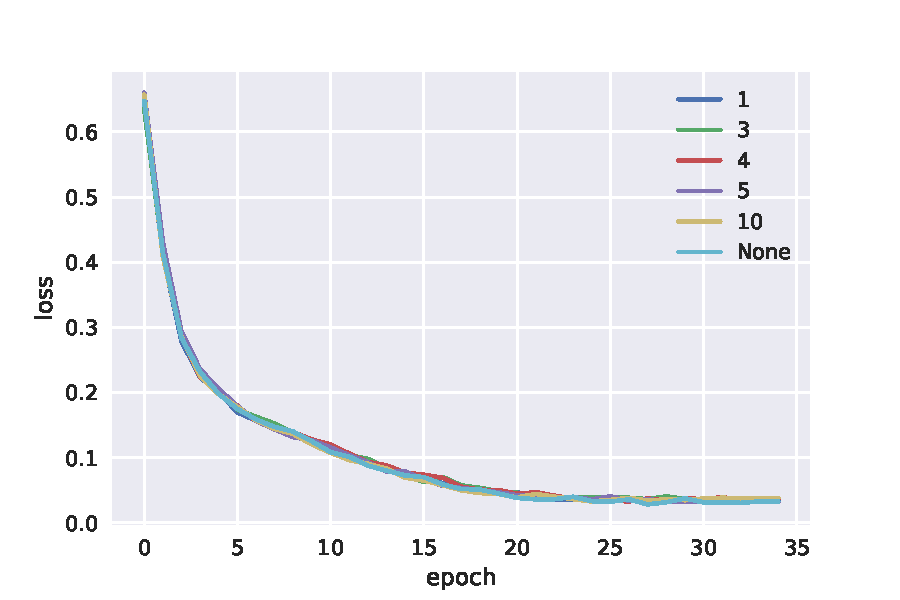
\includegraphics[width=\textwidth]{./figures/results/decay/losses.pdf}
    \caption{The average loss at each epoch.\\}%
    \label{fig:decay_loss}
  \end{subfigure}
  \begin{subfigure}[t]{0.49\textwidth}
    \centering
    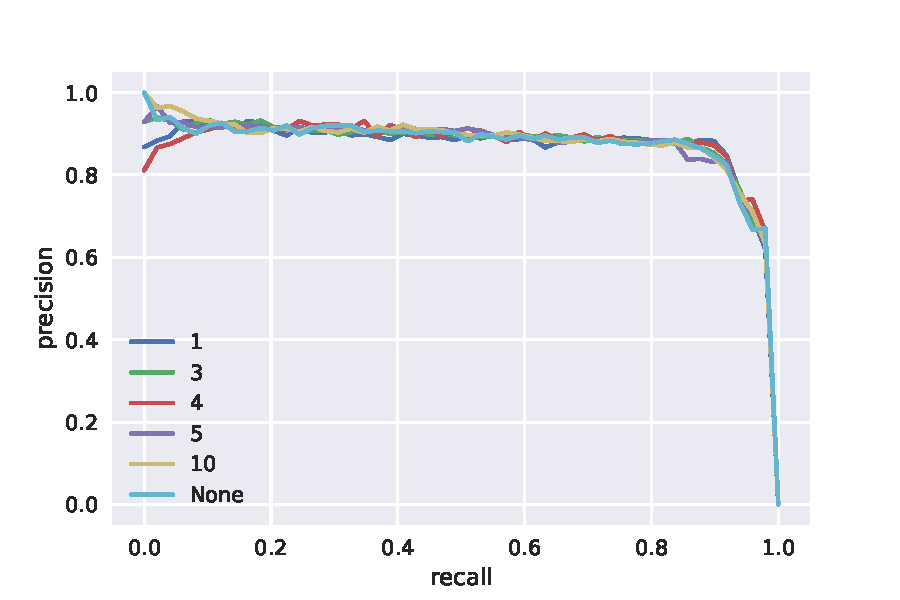
\includegraphics[width=\textwidth]{./figures/results/decay/pr.pdf}
    \caption{The average precision-recall curves at various decay values.}%
    \label{fig:decay_pr}
  \end{subfigure}
  \caption{The loss over time (\subref{fig:decay_loss}) and the
    precision-recall curve (\subref{fig:decay_pr}). In both cases, the values are
    averaged over 10 trials.}%
    \label{fig:decay_plots}
\end{figure}

\begin{figure}[htbp]
  \centering
  \begin{subfigure}[t]{0.49\textwidth}
    \centering
    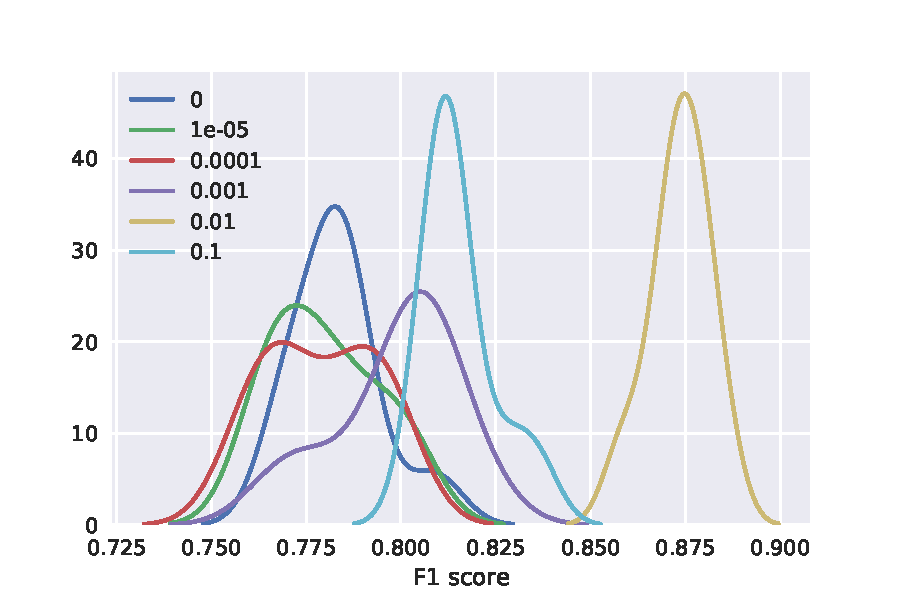
\includegraphics[width=\textwidth]{./figures/results/decay/kde_f1.pdf}
    \caption{Kernel density estimation}%
    \label{fig:decay_kde}
  \end{subfigure}
  \begin{subfigure}[t]{0.49\textwidth}
    \centering
    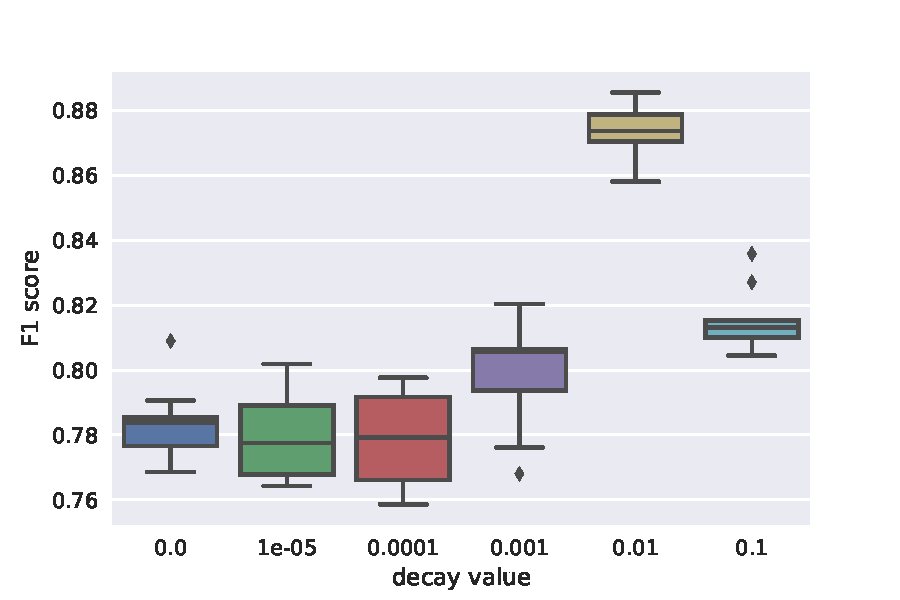
\includegraphics[width=\textwidth]{./figures/results/decay/boxplot_f1.pdf}
    \caption{Boxplot}%
    \label{fig:decay_box}
  \end{subfigure}
  \caption{A kernel density estimation and boxplot, based on the F1 score values
  over 10 repeated trials.}%
  \label{fig:decay_dists}
\end{figure}

\begin{table}[htb]
  \centering
  \import{./figures/results/decay/}{f1_sign.tex}
  \caption{\emph{p}:-Values for the decay parameter. Each value between two
    distributions of F1 scores indicates the probability of both populations
    being generated from the same distribution distribution.}%
  \label{tbl:decay_p}
\end{table}

\begin{table}[htb]
  \centering
  \import{./figures/results/decay/}{scores.tex}
  \caption{The F1 and AoC scores at various decay values.}%
  \label{tbl:decay}
\end{table}

\FloatBarrier%

%%% Local Variables:
%%% mode: latex
%%% TeX-master: "report"
%%% End:
